\subsubsection{Sistema de autorregulación de temperatura}

Para elevar la temperatura dentro del contenedor, se propuso realizar en forma de inducción utilizando un modelo basado en el de parrillas de resistencias eléctricas (Figura \ref{fg:parrilla}). 

\begin{figure}[h!]
            \centering
            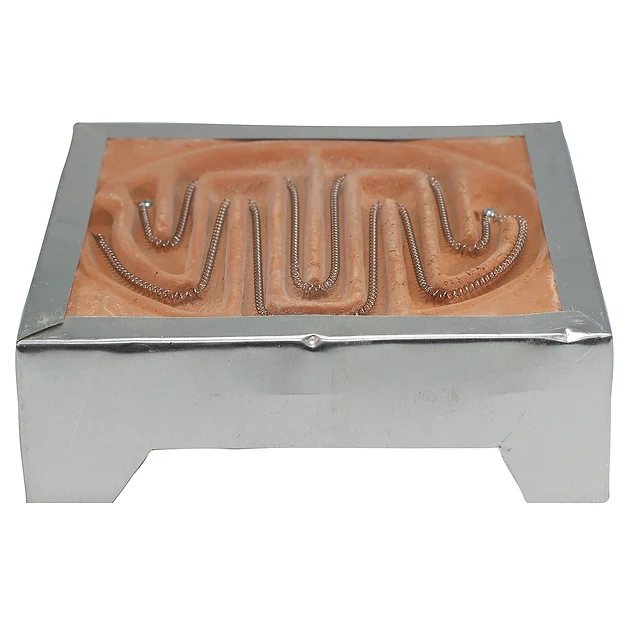
\includegraphics[scale=0.25]{images/Capitulo 4/s5/res.png}
            \caption{Parrilla para elevar la temperatura}
            \label{fg:parrilla}
        \end{figure}

Para elevar la temperatura, se colocaron dos parrillas al fondo del contenedor, como se ve en el trabajo de Rodriguez D. \cite{David2016}. De esta forma la transferencia de calor va de abajo hacia arriba por lo que se puede tener una transmisión mas uniforme. 

Estas parrillas utilizan un elemento calefactor, el cual es un elemento que es capaz de convertir la energía eléctrica en calor, mediante un proceso resistivo, también conocido como el calentamiento de Joule. \cite{calefactor}

Estos elementos suelen estar conformados por bobinas o elementos de alambre, los cuales son susceptibles de calentarse bastante, por lo que produce calor en todas las direcciones.

Se planteo utilizar una resistencia en espiral (Figura \ref{fg:resorte}), hecha con un alambre de aleación Ni-Cr, que usualmente tiene un diámetro de 5mm \cite{resisresorte}. De esta forma, obtenemos una fuente de inducción de calor, también este tipo de resistencias son muy accesibles y económicas. 

\begin{figure}[h]
            \centering
            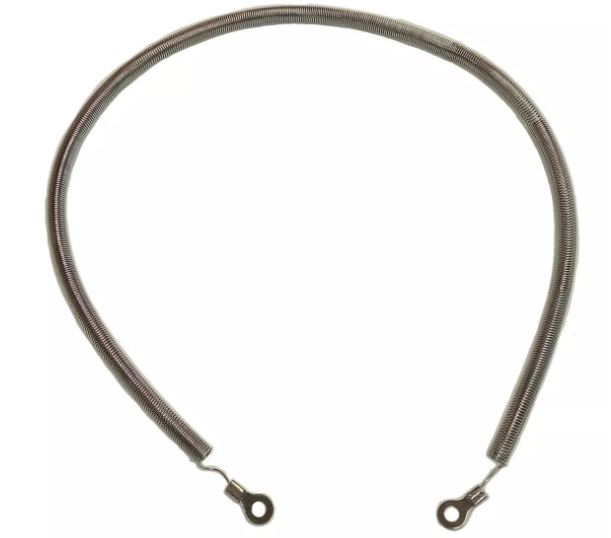
\includegraphics[scale=0.25]{images/Capitulo 4/s5/Res resorte.png}
            \caption{Resistencia tipo resorte}
            \label{fg:resorte}
        \end{figure}

%Esta resistencia esta cubierta por una base de barro, que también suele ser sustituida por una base de ladrillo rojo, esta con el fin de no permitir la conductividad eléctrica además cuenta con una base de aluminio que ayuda a disipar el calor generado.

Para su instalación, se adaptó el modelo de las resistencias a las dimensiones del dispositivo para aprovechar los espacios que se tiene a los costados del contenedor (Figura \ref{fg:Temper_sis}), con el fin, de repartir mejor el calor generado. 

Para su contracción, se utilizo un perfil L de  2x2 in y con un espesor de 0.25 in, sobre el que se le colocó una base de arcilla, material que se parece mucho al ladrillo con el que están echas las parrillas convencionales. 

La arcilla de coloco formando un triangulo con una diagonal recta que une las 2 orillas del perfil. En el punto medio de esta diagonal se realizo una incisión que forma una cavidad de 4 mm de profundidad para colocar ahí la resistencia.

\begin{figure}[h!]
            \centering
            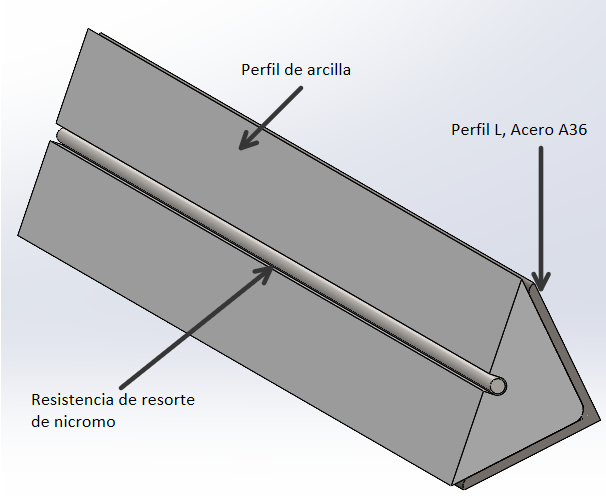
\includegraphics[scale=0.5]{images/Capitulo 4/s5/Sis_termico.png}
            \caption{Modelo físico del sistema de regulación de temperatura}
            \label{fg:Temper_sis}
        \end{figure}

La arcilla sirve como un soporte para la resistencia eléctrica y a su vez sirve como aislante de calor para los materiales de la estructura. De esta manera, las resistencias se colocaron a los costados del contenedor, entre la base que lo sostiene y la estructura del sistema de compostaje.

